\documentclass[a4paper,11pt]{article} %, landscape report

\usepackage[T1]{fontenc}
\usepackage[utf8x]{inputenc}

%Selon les goûts: times palatino bookman newcent chancery helvet avant fourier kpfonts cmbright
%\usepackage{avant}

%\usepackage[hmargin=2cm,vmargin=2cm]{geometry}
%\usepackage{multicol}
%\setlength{\columnsep}{1cm}

\usepackage{graphicx}
\usepackage{xcolor}
\usepackage{multicol}\setlength{\columnsep}{1cm}

\usepackage{amsmath,amssymb,amsfonts,makeidx}
\usepackage{stmaryrd}% crochets «intervalles d'entiers»
%\newcommand{\B}{\mathbb{B}}
\usepackage{tikz}
\newcommand{\e}{\text{e}}

\usepackage{lscape}

\newcommand{\vesp}{\vspace*{0.2em}}
\newcommand{\VESP}{\vspace*{0.8em}}
\newcommand{\ttt}[1]{\texttt{#1}}
\newcommand{\code}[1]{\colorbox{gray!15}{\texttt{#1}}}
\newcommand{\rem}[1]{\colorbox{yellow}{\textbf{#1}}}


\usepackage{hyperref}
\hypersetup{colorlinks=true,
            linkcolor=violet,
            urlcolor=teal,
            citecolor=olive,
            }
\newcommand{\www}[2]{\href{#1}{\nolinkurl{#2}}}
%black, blue, brown, cyan, darkgray, gray, green, lightgray, lime, magenta, olive, orange, pink, purple, red, teal, violet, white, yellow
%\urlstyle{same}% Pas stylés \og URL

%\usepackage[nosort]{cite}

%\usepackage{minted}
%\usemintedstyle{%friendly, %colorful, %autumn
%    breaklines, fontfamily=courier,%helvetica,%tt,
%    bgcolor=gray!10,
%    %framesep=2mm,
%    %fontsize=\large,
%    %frame=lines,%single,
%    numbers=none,%left,
%    autogobble, mathescape, texcomments,
%    %stepnumber=2,
%    escapeinside=\%
%}
%% Inline
%\newcommand{\Py}[1]{\mintinline[bgcolor=gray!15]{python}{#1}}
%\newcommand{\BPy}[1]{\textbf{\Py{#1}}}
%\newcommand{\SerreCode}{\vspace*{-0.8em}}
\newcommand{\Py}[1]{\colorbox{gray!20}{\texttt{#1}}}

%\newcommand{\1}{\textcircled{\small 1}}
%\newcommand{\2}{\textcircled{\small 2}}
\setlength{\parskip}{0.2em}
%\setlength{\parindent}{0ex}

\usepackage[french]{babel} \frenchbsetup{StandardLists=true}
\usepackage[autolanguage]{numprint}
\DecimalMathComma

\AddThinSpaceBeforeFootnotes
\FrenchFootnotes

% =================================================================================================
%\title{Projet d'initiation à la Recherche\\M2 I2A}
%\author{Jean-Marc Gervais\\[0.6em]
%Encadré par M. Jean-François Couchot\\
%\small Institut FEMTO-ST, UMR 6174 CNRS -- DISC Équipe AND}
%\date{$15$ janvier $2\,020$}

\begin{document}%\setlength\parindent{5mm}
%\maketitle
%%
%\section*{\center Notes...\\[1cm]pytorch-dp}
%%
%\thispagestyle{empty}
%\newpage
%%
%\tableofcontents
%\newpage
\section{Deep Learning}
Exposons quelques points-clés nécessaires pour appréhender ce concept, sans justifier les propriétés citées et en illustrant les concepts dans le cadre de la classification d'images numériques matricielles, en version supervisée: les catégories sont connues dès le départ, ainsi qu'un ensemble de correspondance \og images $\mapsto$ catégorie\fg{} utilisées pour l'apprentissage.
%
\subsection{Neurone formel}
%
Inspiré par la biologie, ce concept a été introduit en $1\,943$ par Warren McCulloch et Walter Pitts. Les stimuli en entrée sont remplacés par des valeurs numériques $x_k$ ($k=1,~...~, n$), affectées chacune d'un poids $w_k$. Le neurone en effectue la somme pondérée, en ajoutant un éventuel biais constant $w_0$. Enfin, il lui applique une fonction dite d'activation (ou de sortie), non linéaire, qui assure un effet de seuil (variation rapide quand la variable franchit une valeur donnée). Parmi celles qui sont couramment utilisées, citons la sigmoïde $\sigma(x)=\frac{1}{1+\e^{-x}}$, la tangente hyperbolique $\tanh(x)=\frac{\e^{x}-\e^{x}}{\e^{x}+\e^{x}}$ et la fonction ReLU (\emph{Rectified Linear Unit}) $f(x)=max(0;x)$.
\begin{center}
    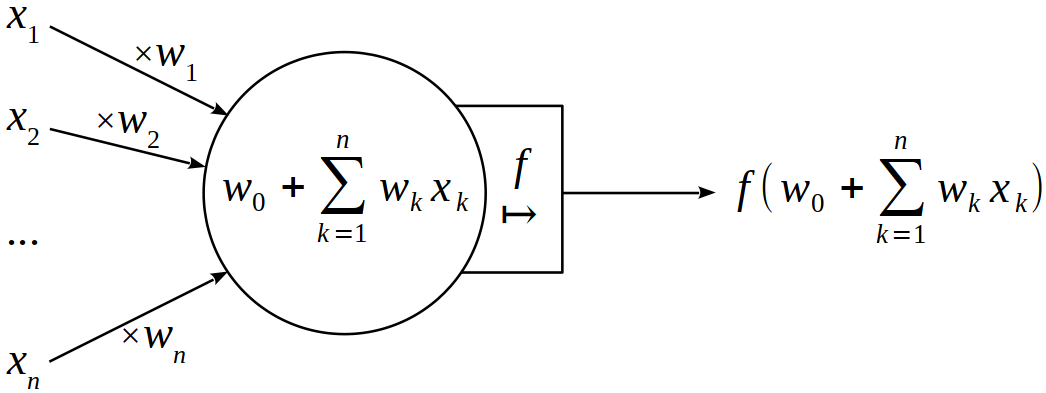
\includegraphics[width=0.7\linewidth]{neurone.png}
\end{center}
%
\subsection{Réseau de neurones}
%
On constitue des couches successives de neurones, dont les sorties sont connectées aux entrées de ceux de la couche suivante.  L'utilisation d'une fonction d'activation non linéaire est nécessaire pour dépasser la capacité d'un unique neurone et pouvoir résoudre des problèmes non linéaires.

Les données à analyser comme les pixels d'une image forment la couche d'entrée. Suivent des couches dites cachées ---~la profondeur dans \og \emph{deep learning}\fg{} faisant référence à leur nombre~--- et enfin la couche de sortie, où chaque neurone est associé à une étiquette dans les problèmes de catégorisation d'images: plus la valeur en sortie du neurone est élevée, plus la catégorie associée est supposée être probable.
\begin{center}
    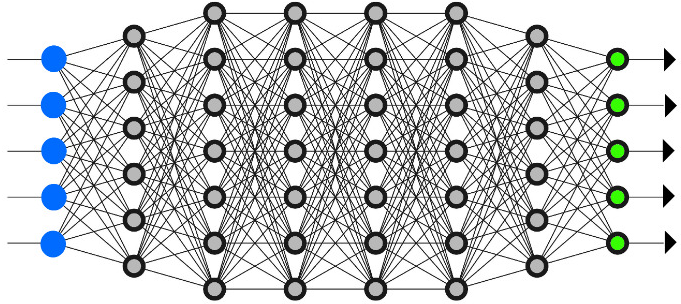
\includegraphics[width=0.7\linewidth]{deep-learning.png}
\end{center}
%
\subsection{Apprentissage automatique par rétropropagation}
%
Sur le jeu de données fourni (\emph{dataset}) , une partie importante servira à l'apprentissage, mais on en conserve une partie à part, pour pouvoir réaliser des tests sur des images nouvelles afin de détecter le sur-apprentissage (\emph{overfitting}. Ce phénomène traduit l'utilisation par le réseau de caractéristiques trop spécifiques aux cas utilisés en phase d'apprentissage, ce qui induit une baisse des performances sur de nouvelles entrées.

Ainsi, on initialise le réseau avec des pondérations aléatoires, puis on l'entraîne sur les images étiquetées en ajustant ses pondérations afin d'améliorer l'exactitude en sortie, tout en vérifiant régulièrement que cette dernière ne diminue pas sur les données de test non utilisées dans la phase précédente.

La méthode de \textbf{rétropropagation du gradient}, introduite par Paul Werbos en $1\,974$ et mise au point douze ans plus tard par David Rumilhart, donne leur puissance aux réseaux multicouches\footnote{La quatrième vidéo YouTube de 3blue1brown décrit progressivement les calculs en détail, sur un exemple simple, \url{https://frama.link/backprop}}:
\begin{itemize}
    \item
    Une image est donnée en entrée au réseau.
    \item
    Les valeurs des neurones obtenues en sortie sont comparées à celles attendues. On évalue les écarts à l'aide d'une fonction d'erreur qu'on cherche à minimiser.
    \item
    On modifie légèrement les pondérations en entrée de chaque neurone de la dernière couche en appliquant une méthode de descente de gradient, de manière à minimiser la fonction d'erreur précédente.
    \item
    L'enchaînement des calculs des différentes couches est une fonction composée, on peut donc évaluer l'impact des variations de chacune des pondérations sur les suivantes.
    On remonte ainsi récursivement jusqu'aux poids des neurones de la première couche cachée, en ajustant au mieux les coefficients à chaque niveau pour minimiser l'erreur en sortie. C'est la phase dite de rétropropagation du gradient.
    \item
    On recommence, pour affiner les réglages, tout en surveillant le taux de reconnaissance sur le jeu de test: si ce dernier tend à diminuer, on termine la phase d'apprentissage pour éviter l'\emph{overfitting}.
\end{itemize}

En fait, on \og nourit \og généralement l'algorithme avec un certain nombre d'images avant de mettre à jour les paramètres du modèle. Ainsi, on dit qu'on forme un lot (\emph{batch}), dont la taille est l'un des hyper-paramètres\footnote{On distingue par ce terme les réglages généralement fixes de l'algorithme, de ceux du modèle qu'il construire et qui évolueront au fur du déroulement.} de l'algorithme. Quand on a soumis toutes les données du \emph{training dataset} à l'algorithme, on dit qu'on a terminé une \emph{epoch} (une période en quelque sorte, mais généralement le terme n'est pas traduit dans les écrits francophones). Ainsi, on distingue plusieurs variantes d'algorithmes\footnote{\emph{Cf.} \href{https://machinelearningmastery.com/gentle-introduction-mini-batch-gradient-descent-configure-batch-size/}{https://machinelearningmastery.com/gentle-introduction-mini-batch-gradient- descent-configure-batch-size}}:
\begin{itemize}
    \item
    \textbf{SGD, \emph{Stochastic Gradient Descent}}, quand une unique image, aléatoire, est soumise avant de mettre à jour les paramètres du modèle (\emph{batch size} de $1$).
    \item
    \textbf{Batch}, quand le lot est constitué de la totalité des données d'entraînement.
    \item
    \textbf{Mini-batch} pour les cas intermédiaires, où la \emph{batch size} est strictement comprise entre $1$ et la taille du \emph{training dataset}. Il y a donc plusieurs mises à jour des paramètres du modèle, une après l'analyse des sorties associées à chaque lot, pour une \emph{epoch} donnée.
\end{itemize}

La programmation des calculs associés à la mise à jour des paramètres est vite fastidieuse. Par ailleurs, elle revient systématiquement dans ces réseaux profonds et peut se paralléliser. Plusieurs \emph{frameworks} les ont donc implémentés, tout en tirant partie des capacités de calculs des GPU. L'outil proposé par Facebook Research, \ttt{PyTorch}, est arrivé plus tardivement que \ttt{TensorFLow}  (Google) par exemple. Mais son succès semble grandissant et l'un des intérêts est d'offrir un calcul transparent du gradient: il suffit d'enregistrer au fur et à mesure les opérations effectuées à chaque étape dans la phase directe, des entrées aux sorties. Ensuite, l'ajustement des paramètres est effectué automatiquement à la demande (\ttt{autograd}).
%%
\section{Réseaux de neurones convolutifs}
%%
On a occulté jusqu'ici la préparation des données en entrée, spécifique à chaque format et importante pour obtenir de bons résultats. Les CNN, \emph{Convolutional Neural Network} ou réseau de neurones convolutifs, constituent une évolution du réseau neuronal multicouche basique, particulièrement adaptée au traitement des images, car il inclut une forme de pré-traitement. Le français Yann Le Cun en a été le pionnier.\\
\begin{center}
	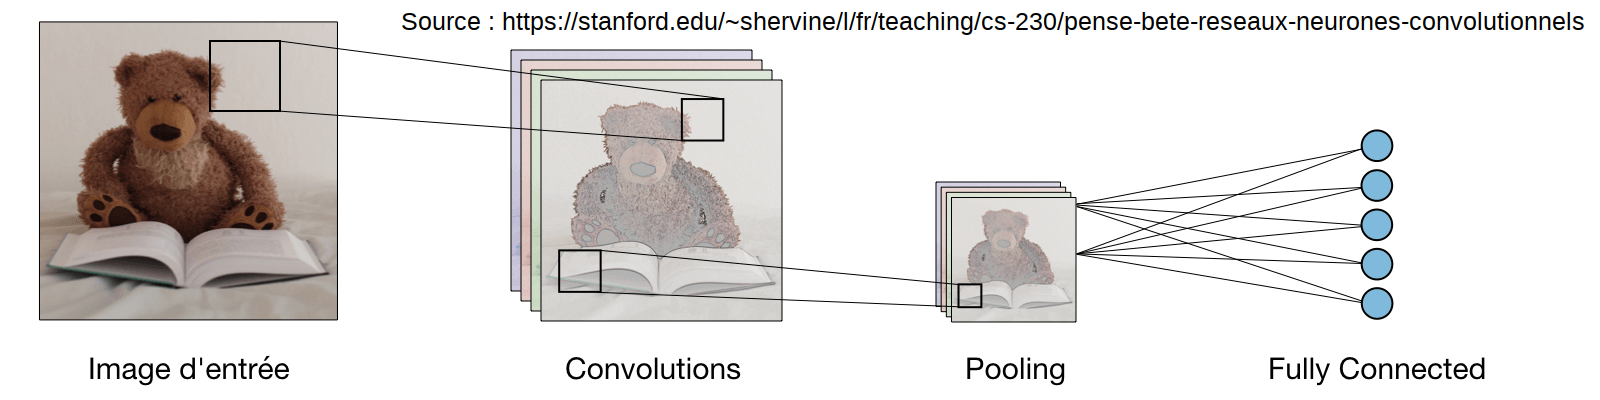
\includegraphics[width=\linewidth]{architecture-cnn.png}
\end{center}
\begin{itemize}
	\item
	Les premières couches dites convolutionnelles (\emph{convolutional layers}) donnent leur nom aux CNN. Elles ont pour but de \og faire apparaître\fg{} des motifs exploitables dans les données de départ. On parle également de \emph{feature map} ou \emph{activation map}.\\
	En entrée on trouve la grille des pixels d'une image (la \og profondeur\fg{}, nombre de canaux ou \emph{channels} est de $1$ pour ces images monochromes, de $3$ pour du RGB, etc.) Un filtre (ou \emph{kernel}) constitué d'un tenseur de petite taille balaye l'image (ou les données précédentes) en entrée, en leur appliquant un produit terme à terme, pour produire une couche suivante en sortie. Si la profondeur est supérieure à $1$ en entrée, on additionne les valeurs obtenues pour chaque canal. On peut ajouter une éventuelle valeur constante qualifiée de biais. En fait, on peut même traiter ce nombre comme un poids parmi les autres, associé à un pseudo-neurone de valeur constante, ce qui est fait pour se ramener à des produits matriciels, en interne.\\
	Le pas du décalage du point d'application du filtre sur l'image en entrée, d'une étape à la suivante (\emph{stride}, à $1$ par défaut, suivant chaque dimension), ainsi que la taille des marges remplies de $0$ ajoutées autour de la matrice d'entrée (\emph{padding}, par défaut à $0$) peuvent être précisées.
	\begin{center}
		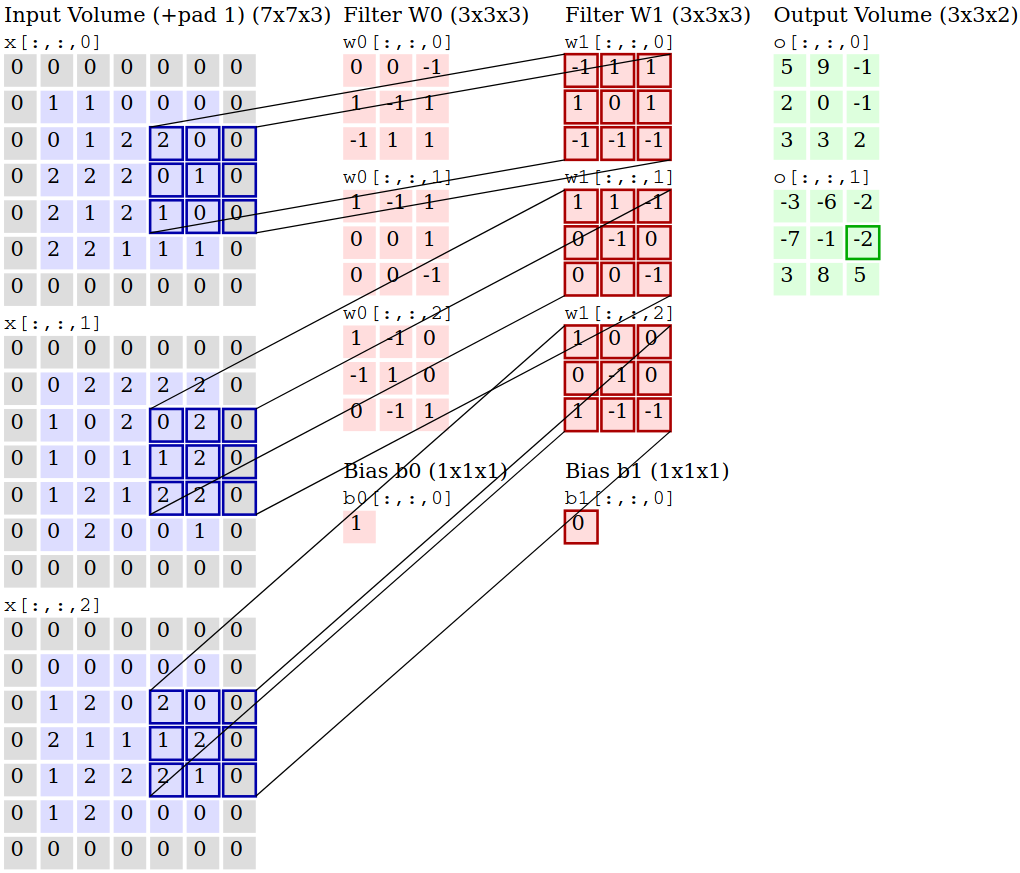
\includegraphics[width=\linewidth]{convolution.png}
	\end{center}
    Si l'on souhaite une profondeur multiple en sortie, on utilise un \emph{kernel} à plusieurs canaux, chacun agissant comme un filtre indépendant qui fournit un niveau de profondeur en sortie. Il y en a deux notés W0 et W1 sur l'illustration précédente\footnote{Source: image animée sur \url{https://cs231n.github.io/convolutional-networks/}}.\\
	\item
	On prolonge souvent les convolutions par un \emph{pooling}, qui permet de regrouper les valeurs de pixels voisins pour sous-échantillonner et  réduire la taille des données à traiter. Traditionnellement, on procède en remplaçant des groupes carrés (ou rectangulaires) de pixels de petites dimensions par leur maximum ou leur moyenne, en balayant là aussi les images ou données en entrée comme pour les convolutions.\\
	Là encore, on peut choisir des \emph{stride} et \emph{padding} spécifiques ou conserver les valeurs par défaut.\footnote{Les deux illustrations suivantes proviennent respectivement de\\ \url{https://pathmind.com/wiki/convolutional-network} et de\\ \url{http://stanford.edu/~shervine/l/fr/teaching/cs-230/pense-bete-reseaux-neurones-convolutionnels}}
	\begin{center}
		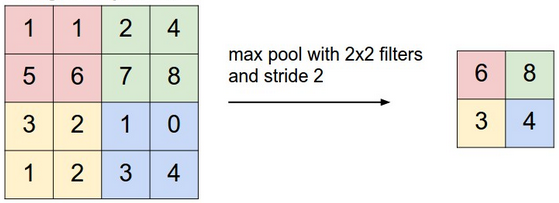
\includegraphics[width=0.6\linewidth]{pooling.png}
	\end{center}
   Notons qu'on peut enchaîner plusieurs étapes de convolutions/\emph{poolings} avant de passer à l'étape suivante.
	\item
	On termine par les couches complètement connectées (\emph{fully connected layers}) d'un perceptron classique, avec au final les sorties associées à chacune des catégories à pronostiquer, les $10$ chiffres dans le cas qui nous concerne.
	\begin{center}
		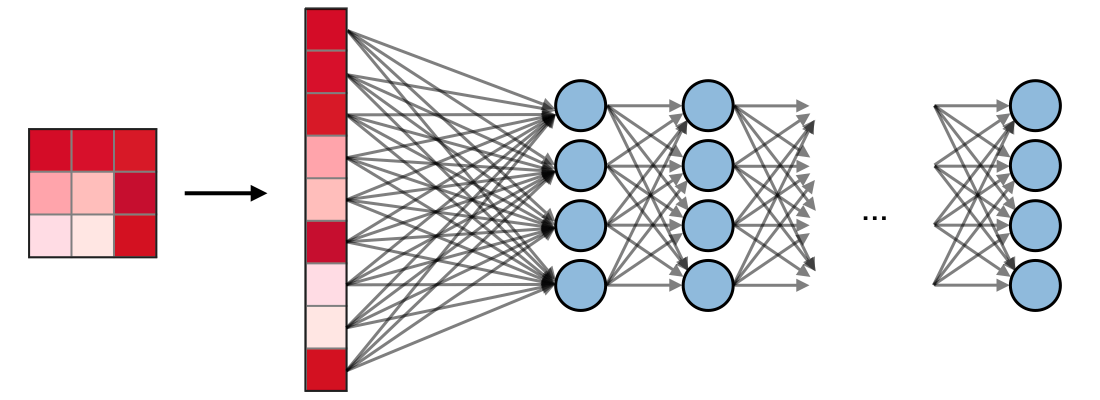
\includegraphics[width=0.8\linewidth]{fully-connected.png}
	\end{center}
\end{itemize}
\subsection{Exemple du MNIST}
Le MNIST\footnote{\url{http://yann.lecun.com/exdb/mnist/}} est une base d'images de chiffres manuscrits associés à leur valeur numérique ($60\,000$  d'entraînement et $10\,000$ de test), devenue une référence en matière de reconnaissance d'images.

\subsubsection{Projet étudié}
Dans la suite, on considère \url{github.com/facebookresearch/pytorch-dp}, sans se préoccuper de préservation de la confidentialité dans un premier temps.

Le projet s'installe classiquement via\\\ttt{git clone https://github.com/facebookresearch/pytorch-dp.git},\\ puis depuis le répertoire \ttt{pytorch-dp} créé:\quad \ttt{pip3 install -e . }\footnote{Testé sous Debian 10.3 vierge ---~environnement de bureau et utilitaires systèmes inclus lors de l'installation~---, après installation des paquets \ttt{git} et \ttt{python3-pip}; utilisation de \ttt{pip3} au lieu de \ttt{pip} indiqué sur le dépôt GitHub, pour travailler avec Python3. Il a fallu allouer au moins 2,5Go de RAM à la machine virtuelle utilisée, le temps de l'installation}

Le réseau est une instance de la classe \ttt{SampleConvNet} (fichier \ttt{mnist.py} du dossier \ttt{examples}) qui hérite de \ttt{nn.Module}, où \ttt{nn} est l'alias habituel pour \ttt{torch.nn} qui sert de base aux divers réseaux neuronaux dans \textsf{PyTorch}.

\subsubsection{Structure du réseau de neurones}
Chacune des entrées sera une image en niveaux de gris de $28\times28$ pixels (normalisée au préalable). Le constructeur crée deux couches convolutives, suivies d'une couche classique \emph{fully connected} qui aboutit en sortie aux $10$ neurones associés à chacun des chiffres à identifier. La méthode \ttt{forward()} qui s'exécutera à chaque \emph{epoch}, autrement dit à chaque itération du processus d'apprentissage, définit les transitions d'une couche à la suivante.
\begin{itemize}
	\item
	Chaque image du \emph{batch} est transformée par convolution avec un \emph{kernel} (un filtre) de dimension $8\times8$ et qui parcourt l'image par pas de $2$ (\emph{stride}) suivant chacune de ses dimensions, sans \emph{padding}. Il a une profondeur de $16$ et produit donc en sortie une couche de $11\times11$ sur $16$ \emph{channels}\footnote{Voir les explications sur le schéma général. Idem pour les dimensions suivantes}
    (\emph{cf.} \Py{self.conv1 = nn.Conv2d(1, 16, 8, 2)} dans le constructeur).
	\item
	En sortie, la non-linéarité est assurée par la fonction ReLU (\emph{Rectified Linear Unit}) qui se réduit à l'identité sur l'ensemble des positifs et à la fonction nulle pour les négatifs. Les valeurs sont alors sous-échantillonnées par un \og max-\emph{pooling}\fg{} de $2\times2$, d'où les dimensions $10\times10$ en sortie
    (\Py{x = F.relu(self.conv1(x))} puis\\\Py{x = F.max\_pool2d(x, 2, 1)} dans la méthode \ttt{forward()}).
	\item
	La seconde convolution est associée à un \emph{kernel} de $4\times4$ et de profondeur $32$, appliqué par pas de $2$ sans \emph{padding}, d'où la dimension $4\times4$ de la couche suivante (\Py{self.conv2 = nn.Conv2d(16, 32, 4, 2)} dans le constructeur).
	\item
	Cette dernière subit à nouveau un max-\emph{pooling} $2\times2$ sans \emph{padding}, pour arriver à une couche en $3\times3$ de profondeur $32$ (\emph{commandes similaires}).
	\item
	Ces données sont remises \og à plat\fg{} sous forme d'un vecteur de taille $32\times3\times3$. Ce dernier est enfin relié aux $10$ neurones de la couche visible de sortie, en mode \emph{fully connected} comme dans un réseau de neurone basique (\Py{self.fc1 = nn.Linear(32 * 3 * 3, 10)} dans le constructeur, et \Py{x = x.view(-1, 32 * 3 * 3)}, puis \Py{x = self.fc1(x)} dans \ttt{forward()}).
\end{itemize}
%
%\begin{landscape}
    \hspace*{-0.3\textwidth}
	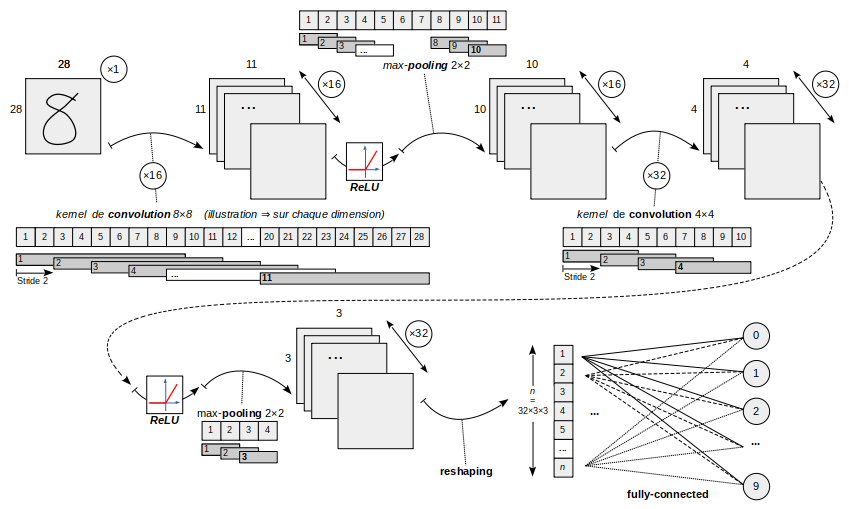
\includegraphics[width=1.6\textwidth]{cnn.png}
%\end{landscape}

\subsubsection{Déroulement du script}
Après avoir pris en compte les éventuels paramètres passés lors de l'appel, la fonction \ttt{main()} crée deux instances de \ttt{torch.utils.data.Dataloader}, des itérables sur les \emph{datasets} d'entraînement et de test, respectivement.

Ensuite, le réseau de neurones est instancié, l'optimisation basée sur une SGD (c'est à ce stade que la méthode est adaptée pour y injecter la garantie de confidentialité différentielle, nous y reviendrons), puis la phase d'entraînement assuré par la fonction \ttt{train()} répétée \ttt{epochs} fois. Enfin, la fonction \ttt{test()} évalue  l'état du réseau obtenu. Ce bloc d'instructions est répété éventuellement \ttt{n\_runs} fois et c'est la moyenne des résultats qui est prise en compte au final et affichée (voire sérialisée sur disque suivant les paramètres).\\[0.4em]

Plus précisément, \ttt{train()}
\begin{itemize}
    \item
    Passe le réseau de neurone en \og mode entraînement\fg{}
    \item
    Choisit la fonction d'évaluation des pertes (\ttt{CrossEntropyLoss()} ici, soit un \ttt{LogSolftmax()} ---~où le logarithme assure un meilleur étagement des valeurs et évite d'atteindre les limites de la représentation des flottants quand on est trop proche de zéro d'où une meilleure compatibilité avec la SDG~--- suivi d'une \emph{Negative Log Likehood} \ttt{NLLLoss()} qui donne en sortie l'indice d'une des classes).
    \item
    Pour chaque \emph{batch} des données d'entraînement: réinitialise les gradients, évalue les pertes sur les exemples, et la applique la rétropropagation du gradient pour mettre à jour les paramètres~--- la méthode \ttt{backward} assure automatiquement ce calcul, c'est l'un des principaux atouts d'un \emph{framework}  comme \textsf{PyTorch}.
\end{itemize}

La fonction \ttt{test()}, quant à elle choisit le mode \og évalutation\fg{}, puis procède de manière analogue sur le jeu de test, mais sans \og suivi\fg{} par \textsf{PyTorch} du gradient, puisqu'il n'y a pas de rétropropagation de gradient à effectuer. En sortie du réseau de neurones, on obtient pour chacune des images testées les probabilités estimées pour chaque chiffre (dans \ttt{output=model(data)}) puis lequel est prédit (via \ttt{argmax}, résultat dans \ttt{pred}). Les statistiques sont alors affichées.


\section{Confidentialité différentielle dans \ttt{mnist.py}}
La prise en compte des opérations garantissant la confidentialité différentielle (DP, \emph{differential privacy}) n'intervient qu'en deux endroits dans \ttt{mnist.py}, à savoir dans les blocs des \Py{if not args.disable\_dp:}

Le premier est dans la fonction \ttt{train()}. C'est un ajout facultatif, pour récupérer puis présenter, en plus de ce qui est affiché en version standard, les paramètres $\epsilon$, $\delta$ et $\alpha$. L'autre constitue la partie incontournable, qui sera à reprendre pour adapter \ttt{pytorch-dp} à d'autres \emph{datasets}. Elle se situe dans \ttt{main}. Il s'agit de remplacer l'\emph{optimizer} \ttt{SGD} standard par sa version DP-compatible.

%
\rem{Repousser plus loin le lien avec la théorie / Rényi-DP et ses coeff. ?}\\
\rem{Ou au contraire, commencer au moins par qualifier les paramètres ?}
%
Un objet de la classe \ttt{PrivacyEngine} (\emph{cf.} \ttt{privacy\_engine.py}) est créé, ce qui permet de préciser les paramètres concernant la DP, notamment la liste \ttt{alpha} des coefficients $\alpha$, ici $1,1$; $1,2$; $1,3$; ...~; $10,9$ puis $12$; $13$; ...~; $63$, ou le seuil \ttt{max\_grad\_norm} de \emph{clipping} des normes des gradients. Puis, grâce à la méthode \ttt{attach()}
 d'un tel objet, de remplacer l'\emph{optimizer} du réseau de neurones par sa version DP. En particulier, sa méthode \ttt{step()} est modifiée, et il expose \ttt{get\_privacy\_spendt()} qui permet de suivre le budget de confidentialité (\emph{cf. partie incluse dans \ttt{train()}}).

%
\rem{détailler le rôle des argu. ? Et donc intérêt / explication théorique avant...}\\
%

\rem{Détailler les autres méthodes : get\_etc. et step() surtout.}
\section{\texttt{pytorch-dp}}
Le dossier \ttt{torchdp} contient ce qui assure  la DP: ajout de bruit, décompte du budget de confidentialité.
\begin{itemize}
	\item
	\ttt{privacy\_engine.py} définit la classe \ttt{PrivacyEngine}, au cœur du dispositif de DP. Comme on l'a vu, sa méthode \ttt{attach()} permet d'insérer la gestion de la DP dans l'\emph{optimizer} standart passé en paramètre.//
    Ses méthodes \ttt{get\_renyi\_divergence()} et\\ \ttt{get\_privacy\_spent(targetted\_delta)} se chargent des calculs associés en se basant sur les outils de \ttt{privacy\_analysis.py}.\\\rem{détailler leur but // théorie}
	\item
    \ttt{privacy\_analysis.py}, qui reprend le travail de Google TensorFlow Privacy, fournit essentiellement les deux fonctions appelées comme on vient de le voir par \ttt{PrivacyEngine} (les autres n'étant utiles qu'en interne). \rem{Détailler le rôle des param. ?}
    \item
    \ttt{dp\_model\_inspector.py}, qui s'appuie sur la classe \ttt{ModelInspector} de \ttt{utils.py}  et \ttt{per\_sample\_gradient\_clip.py} contiennent deux classes utilisées par \ttt{privacy\_engine.py}.\rem{+ Détailler leurs rôles... +}
    \item
    \ttt{autograd\_grad\_sample.py}\\\rem{À explorer, semble non essentiel pour le fonctionnement}
\end{itemize}
\pagebreak
\section{Notes hors plan du document pour l'instant}
\rem{Pour mémoire, liens entres différentes garanties de DP :}\\
$\varepsilon$-DP\quad $\Rightarrow$ \quad $(\varepsilon, \delta)$-DP\\
$\varepsilon$-DP\quad $\Rightarrow$ \quad
  $(\infty, \varepsilon)$-RDP \quad $\Rightarrow$ \quad
  $(\alpha, \varepsilon)$-RDP\quad $\stackrel{\forall\,0<\delta<1}{\Longrightarrow}$ \quad
  $\left( \varepsilon + \dfrac{\ln{1/\delta}}{\alpha-1}, \delta \right)$-DP\\
\rem{et}\\
$\varepsilon$-DP\quad / Laplace\\
$(\varepsilon, \delta)$-DP\quad / Gauss,\quad faible probabilité  $\delta$ de perte de confidentialité\\
$(\alpha, \varepsilon)$-RDP (Rényi)\quad moment accountant, Gauss / random subsets


\end{document}
